% Methodology figure -- the layered design flow as a block diagram (left),
% parallel to an illustration of what each layer sets on the substrate
% (right): tiles mapped onto the 3D mesh, and a zoom into one node showing
% the port loads (PIL/PEL -> PF, packing-fixed) and the link load
% (Lambda_l -> PL, placement-set).  Concepts only: no result numbers.
% Standalone; pdflatex fig_methodflow.tex -> fig_methodflow.pdf
\documentclass[border=3pt]{standalone}
\usepackage{times}
\usepackage{amsmath}
\usepackage{tikz}
\usetikzlibrary{arrows.meta,positioning,calc,fit,backgrounds}

\definecolor{cPack}{HTML}{2A78D6}   % packing
\definecolor{cMap}{HTML}{EB6834}    % mapping / PL
\definecolor{cRoute}{HTML}{1BAF7A}  % routing
\definecolor{cInk}{HTML}{101720}
\definecolor{cInk2}{HTML}{3A4653}
\definecolor{cFaint}{HTML}{9AA5B1}
\definecolor{cGridL}{HTML}{C9D2DB}

\begin{document}
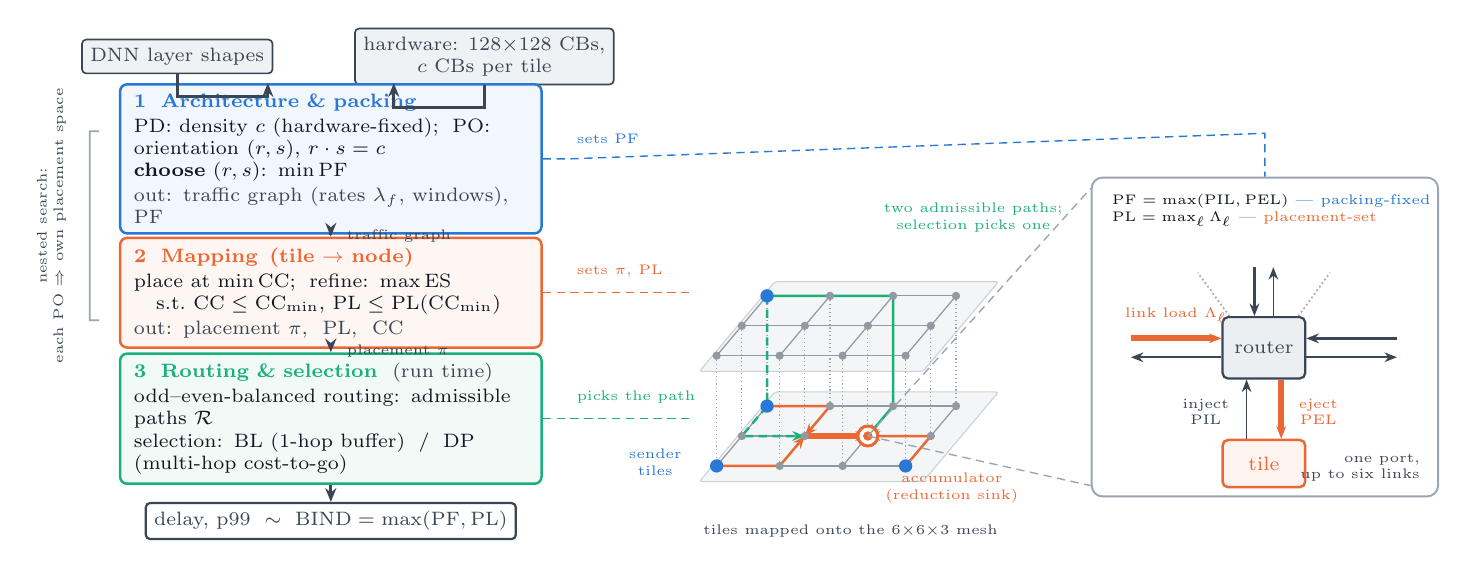
\begin{tikzpicture}[
  font=\scriptsize,
  ar/.style={-{Stealth[length=4.5pt,width=3.5pt]},line width=0.8pt,color=cInk2},
  flow/.style={-{Stealth[length=5pt,width=4pt]},line width=1.0pt,color=cInk2},
  lead/.style={line width=0.5pt,color=cFaint,densely dashed},
  lbl/.style={font=\scriptsize,color=cInk,align=center},
  sub/.style={font=\tiny,color=cInk2,align=center},
  blk/.style={draw,rounded corners=2.5pt,line width=0.9pt,align=left,
              inner xsep=5pt,inner ysep=3.5pt,text width=50mm,font=\scriptsize},
  io/.style={draw,line width=0.6pt,color=cInk2,fill=cGridL!30,rounded corners=1.5pt,
             align=center,inner sep=3pt,font=\scriptsize},
  tag/.style={font=\tiny\bfseries,text=white,inner sep=2pt,rounded corners=1pt},
]

% ====================================================== LEFT: the design flow
% inputs
\node[io] (inDNN) at (0.0,5.35) {DNN layer shapes};
\node[io] (inHW)  at (3.9,5.35) {hardware: $128{\times}128$ CBs,\\$c$ CBs per tile};

% -- layer 1: architecture & packing
\node[blk,color=cPack,fill=cPack!6,text=cInk] (L1) at (1.95,4.05)
  {\textbf{\textcolor{cPack}{1\; Architecture \& packing}}\\[1pt]
   PD: density $c$ (hardware-fixed);\; PO: orientation $(r,s)$, $r\cdot s=c$\\
   \textbf{choose} $(r,s)$: $\min \mathrm{PF}$\\[1pt]
   \textcolor{cInk2}{out: traffic graph (rates $\lambda_f$, windows),\ \ $\mathrm{PF}$}};

% -- layer 2: mapping
\node[blk,color=cMap,fill=cMap!6,text=cInk] (L2) at (1.95,2.35)
  {\textbf{\textcolor{cMap}{2\; Mapping \,(tile $\to$ node)}}\\[1pt]
   place at $\min \mathrm{CC}$;\; refine: $\max \mathrm{ES}$\\
   \quad s.t.\ $\mathrm{CC}\le\mathrm{CC}_{\min}$, $\mathrm{PL}\le\mathrm{PL}(\mathrm{CC}_{\min})$\\[1pt]
   \textcolor{cInk2}{out: placement $\pi$,\ \ $\mathrm{PL}$,\ \ $\mathrm{CC}$}};

% -- layer 3: routing & selection
\node[blk,color=cRoute,fill=cRoute!6,text=cInk] (L3) at (1.95,0.75)
  {\textbf{\textcolor{cRoute}{3\; Routing \& selection}}\ \ \textcolor{cInk2}{(run time)}\\[1pt]
   odd--even-balanced routing: admissible paths $\mathcal R$\\
   selection: BL (1-hop buffer)\; /\; DP (multi-hop cost-to-go)};

% -- output
\node[io,fill=white,line width=0.8pt] (out) at (1.95,-0.55)
  {delay, p99 \;$\sim$\; $\mathrm{BIND}=\max(\mathrm{PF},\mathrm{PL})$};

% flow arrows
\draw[flow] (inDNN.south) -- ++(0,-0.28) -| ($(L1.north)+(-0.8,0)$);
\draw[flow] (inHW.south)  -- ++(0,-0.28) -| ($(L1.north)+(0.8,0)$);
\draw[flow] (L1.south) -- (L2.north) node[midway,right=2pt,sub]{traffic graph};
\draw[flow] (L2.south) -- (L3.north) node[midway,right=2pt,sub]{placement $\pi$};
\draw[flow] (L3.south) -- (out.north);

% nested search bracket
\draw[line width=0.6pt,color=cFaint] ($(L1.west)+(-0.25,0.35)$) -- ++(-0.12,0)
   -- ($(L2.west)+(-0.37,-0.35)$) -- ++(0.12,0);
\node[sub,rotate=90,anchor=south,color=cInk2] at ($(L1.west)!0.5!(L2.west)+(-0.55,0)$)
   {nested search:\\each PO $\Rightarrow$ own placement space};

% ====================================================== RIGHT: the substrate
\begin{scope}[shift={(6.85,0.15)}]
  \newcommand{\nodeat}[3]{({#1*0.80+#2*0.32},{#2*0.38+#3*1.40})}
  % planes
  \foreach \z in {0,1}
    \draw[line width=0.4pt,color=cGridL,fill=cGridL!22,rounded corners=1pt]
      ($(-0.22,-0.20+\z*1.40)$) -- ($(2.62,-0.20+\z*1.40)$) --
      ($(3.58,0.94+\z*1.40)$)  -- ($(0.74,0.94+\z*1.40)$) -- cycle;
  % verticals
  \foreach \i in {0,1,2,3} \foreach \j in {0,1,2}
    \draw[line width=0.4pt,color=cFaint,densely dotted]
      \nodeat{\i}{\j}{0} -- \nodeat{\i}{\j}{1};
  % in-plane links
  \foreach \z in {0,1}{
    \foreach \i in {0,1,2,3} \foreach \j in {0,1}
      \draw[line width=0.45pt,color=cGridL!60!cInk2] \nodeat{\i}{\j}{\z} -- \nodeat{\i}{(\j+1)}{\z};
    \foreach \i in {0,1,2} \foreach \j in {0,1,2}
      \draw[line width=0.45pt,color=cGridL!60!cInk2] \nodeat{\i}{\j}{\z} -- \nodeat{(\i+1)}{\j}{\z};
  }
  % reduction flows converging on the accumulator at (2,1,0) -- hot link (1,1)->(2,1)
  \draw[ar,color=cMap,line width=0.9pt] \nodeat{0}{0}{0} -- \nodeat{1}{0}{0} -- \nodeat{1}{1}{0};
  \draw[ar,color=cMap,line width=0.9pt] \nodeat{0}{2}{0} -- \nodeat{1}{2}{0} -- \nodeat{1}{1}{0};
  \draw[ar,color=cMap,line width=2.0pt] \nodeat{1}{1}{0} -- \nodeat{2}{1}{0};
  \draw[ar,color=cMap,line width=0.9pt] \nodeat{3}{0}{0} -- \nodeat{3}{1}{0} -- \nodeat{2}{1}{0};
  % routing choice from the upper plane: two admissible paths, selection picks
  \draw[ar,color=cRoute,line width=0.9pt]
    \nodeat{0}{2}{1} -- \nodeat{2}{2}{1} -- \nodeat{2}{2}{0} -- \nodeat{2}{1}{0};
  \draw[ar,color=cRoute,line width=0.9pt,densely dashed]
    \nodeat{0}{2}{1} -- \nodeat{0}{2}{0} -- \nodeat{0}{1}{0} -- \nodeat{1}{1}{0};
  % nodes
  \foreach \z in {0,1} \foreach \i in {0,1,2,3} \foreach \j in {0,1,2}
    \fill[color=cInk2!55] \nodeat{\i}{\j}{\z} circle (1.5pt);
  \foreach \px/\py/\pz in {0/0/0, 0/2/0, 3/0/0, 0/2/1}
    \fill[color=cPack] \nodeat{\px}{\py}{\pz} circle (2.4pt);
  \path \nodeat{2}{1}{0} coordinate (acc);
  \draw[line width=1.1pt,color=cMap,fill=white] (acc) circle (3.6pt);
  \fill[color=cMap] (acc) circle (1.7pt);
  % labels
  \node[sub,color=cPack,anchor=east] at (-0.32,0.05) {sender\\tiles};
  \node[sub,color=cMap,anchor=north west,inner sep=1pt] at (2.1,-0.05)
     {accumulator\\(reduction sink)};
  \node[sub,color=cRoute,anchor=south west] at (2.0,2.85)
     {two admissible paths;\\selection picks one};
  \node[sub,anchor=north] at (1.7,-0.62) {tiles mapped onto the $6{\times}6{\times}3$ mesh};
\end{scope}

% ====================================================== ZOOM: one node
\begin{scope}[shift={(11.95,0.3)}]
  % frame
  \node[draw,rounded corners=4pt,line width=0.7pt,color=cFaint,fill=white,
        minimum width=4.4cm,minimum height=4.05cm,anchor=south west] (zoom) at (-0.35,-0.55) {};
  % formulas, top of the frame
  \node[sub,anchor=north west,align=left,text=cInk] at (-0.2,3.42)
    {$\mathrm{PF}=\max(\mathrm{PIL},\mathrm{PEL})$ \textcolor{cPack}{--- packing-fixed}\\
     $\mathrm{PL}=\max_\ell \Lambda_\ell$ \textcolor{cMap}{--- placement-set}};
  % router + tile
  \node[draw,line width=0.8pt,color=cInk2,fill=cGridL!35,rounded corners=2pt,
        minimum width=1.05cm,minimum height=0.78cm] (R) at (1.85,1.35) {router};
  \node[draw,line width=0.9pt,color=cMap,fill=cMap!8,rounded corners=2pt,
        minimum width=1.05cm,minimum height=0.6cm] (T) at (1.85,-0.12) {tile};
  % ports: injection (thin), ejection (thick -- the accumulator's floor)
  \draw[ar,color=cInk2,line width=0.6pt] ($(T.north)+(-0.22,0)$) -- ($(R.south)+(-0.22,0)$);
  \draw[ar,color=cMap,line width=2.2pt]  ($(R.south)+(0.22,0)$)  -- ($(T.north)+(0.22,0)$);
  \node[sub,anchor=east,color=cInk2] at ($(T.north)+(-0.32,0.34)$) {inject\\PIL};
  \node[sub,anchor=west,color=cMap]  at ($(T.north)+(0.32,0.34)$)  {eject\\PEL};
  % in-plane links: W hot, E, N (shorter, to stay clear of the formulas)
  \draw[ar,color=cMap,line width=2.2pt] ($(R.west)+(-1.15,0.12)$) -- ($(R.west)+(0,0.12)$);
  \draw[ar,color=cInk2,line width=0.6pt] ($(R.west)+(0,-0.12)$) -- ($(R.west)+(-1.15,-0.12)$);
  \draw[ar,color=cInk2,line width=0.9pt] ($(R.east)+(1.15,0.12)$) -- ($(R.east)+(0,0.12)$);
  \draw[ar,color=cInk2,line width=0.6pt] ($(R.east)+(0,-0.12)$) -- ($(R.east)+(1.15,-0.12)$);
  \draw[ar,color=cInk2,line width=0.8pt] ($(R.north)+(-0.12,0.62)$) -- ($(R.north)+(-0.12,0)$);
  \draw[ar,color=cInk2,line width=0.6pt] ($(R.north)+(0.12,0)$) -- ($(R.north)+(0.12,0.62)$);
  % vertical (z) links, dotted
  \draw[color=cFaint,densely dotted,line width=0.6pt] ($(R.north west)+(0.1,0)$) -- ++(-0.4,0.55);
  \draw[color=cFaint,densely dotted,line width=0.6pt] ($(R.north east)+(-0.1,0)$) -- ++(0.4,0.55);
  % labels
  \node[sub,anchor=south,color=cMap] at ($(R.west)+(-0.58,0.20)$) {link load $\Lambda_\ell$};
  \node[sub,anchor=north,color=cFaint] at ($(R.north)+(0,0.66)$) {};
  \node[sub,anchor=south east,color=cInk2,align=right] at ($(zoom.south east)+(-0.12,0.08)$)
    {one port,\\up to six links};
\end{scope}

% zoom leaders from the marked accumulator to the frame
\draw[lead] (acc) -- ($(zoom.north west)+(0,-0.15)$);
\draw[lead] (acc) -- ($(zoom.south west)+(0,0.15)$);

% cross-links from flow blocks to the illustration
\draw[lead,color=cPack] (L1.east) -- ++(0.35,0) -- ($(zoom.north)+(0,0.55)$) -- (zoom.north);
\draw[lead,color=cMap]  (L2.east) -- ++(0.35,0) -- (6.55,2.35);
\draw[lead,color=cRoute] (L3.east) -- ++(0.35,0) -- (6.55,0.75);
\node[sub,color=cPack,anchor=south west] at (4.95,4.12) {sets PF};
\node[sub,color=cMap,anchor=south west]  at (4.95,2.42) {sets $\pi$, PL};
\node[sub,color=cRoute,anchor=south west] at (4.95,0.82) {picks the path};

\end{tikzpicture}
\end{document}
